\documentclass[11pt,class=report,crop=false]{standalone}
\usepackage[screen]{../python}

\begin{document}


%====================================================================
\chapitre{Turtle (Scratch with Python)}
%====================================================================

\objectifs{The \ci{turtle} module allows you to easily make drawings in \Python. It's about giving orders to a turtle with simple instructions like \og{}go ahead\fg{}, \og{}turn\fg{}\ldots{} It's the same principle as with \emph{Scratch}, but with one difference: you no longer move blocks, instead you write the instructions.}


%%%%%%%%%%%%%%%%%%%%%%%%%%%%%%%%%%%%%%%%%%%%%%%%%%%%%%%%%%%%%%%%
%%%%%%%%%%%%%%%%%%%%%%%%%%%%%%%%%%%%%%%%%%%%%%%%%%%%%%%%%%%%%%%%

\begin{cours}[The \Python{} turtle]
\index{module!turtle@\ci{turtle}}
\index{turtle}

\index{graphic}

Turtle is the ancestor of \emph{Scratch}! In a few lines you can make beautiful drawings.

\begin{lstlisting}
from turtle import *

forward(100)   # Move forward
left(90)       # Turn 90 degrees left
forward(50)
width(5)       # Width of the pencil
forward(100)
color('red')
right(90)
forward(200)

exitonclick()
\end{lstlisting}

\begin{center}
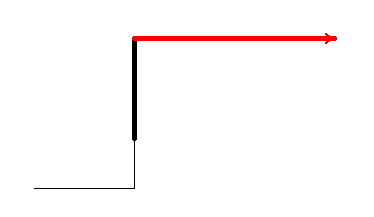
\includegraphics[scale=\myscale,scale=0.6]{screen-turtle-0}
\end{center}

Here is a list of the main commands, accessible after writing:
\mycenterline{\ci{from turtle import *}}

\begin{itemize}
  \item \ci{forward(length)}\index{forward@\ci{forward}} advances a number of steps
  \item \ci{backward(length)} goes backwards
  \item \ci{right(angle)}\index{right@\ci{right}} turns to the right (without advancing) at a given angle in degrees
  \item \ci{left(angle)}\index{left@\ci{left}} turns left
  \item \ci{setheading(direction)} points turtle in a direction ($0$ = right, $90$ = top, $-90$ = bottom, $180$ = left)
  \item \ci{goto(x,y)}\index{goto@\ci{goto}} moves to the point $(x,y)$
  \item \ci{setx(newx)} changes the value of the abscissa
  \item \ci{sety(newy)} changes the value of the ordinate
  
  
  \item \ci{down()}\index{down@\ci{down}} sets the pen down
  \item \ci{up()}\index{up@\ci{up}} sets the pen up
  \item \ci{width(size)} changes the thickness of the line
  \item \ci{color(col)} changes the color: \ci{"red"}, \ci{"green"}, \ci{"blue"}, \ci{"orange"}, \ci{"purple"}\ldots
  
  \item \ci{position()} returns the $(x,y)$ position of the turtle
  \item \ci{heading()} returns the direction \ci{angle} to which the turtle is pointing
  \item \ci{towards(x,y)} returns the angle between the horizontal and the segment starting at the turtle and ending at the point $(x,y)$
  \item \ci{exitonclick()} ends the program as soon as you click
\end{itemize}

The default screen coordinates range from $-475$ to $+475$ for $x$ and
from $-400$ to $+400$ for $y$; $(0,0)$ is in the center of the screen.

\myfigure{0.9}{
  \tikzinput{coord}
}

\end{cours}


%%%%%%%%%%%%%%%%%%%%%%%%%%%%%%%%%%%%%%%%%%%%%%%%%%%%%%%%%%%%%%%%
% Activity 1
%%%%%%%%%%%%%%%%%%%%%%%%%%%%%%%%%%%%%%%%%%%%%%%%%%%%%%%%%%%%%%%%

\begin{activite}[First steps]

\objectifs{Goal: create your first drawings.}

Trace the first letters of \Python{}, for example as below.

\begin{center}
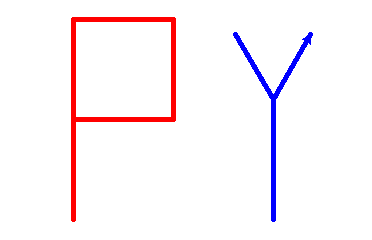
\includegraphics[scale=\myscale,scale=0.4]{screen-turtle-1}
\end{center}

\end{activite}




%%%%%%%%%%%%%%%%%%%%%%%%%%%%%%%%%%%%%%%%%%%%%%%%%%%%%%%%%%%%%%%%
% Activity 2
%%%%%%%%%%%%%%%%%%%%%%%%%%%%%%%%%%%%%%%%%%%%%%%%%%%%%%%%%%%%%%%%

\begin{activite}[Figures]

\objectifs{Goal: draw geometric shapes.}

\begin{center}
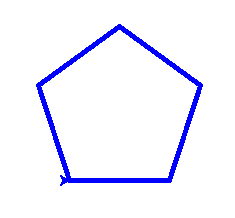
\includegraphics[scale=\myscale,scale=0.25]{screen-turtle-2a}
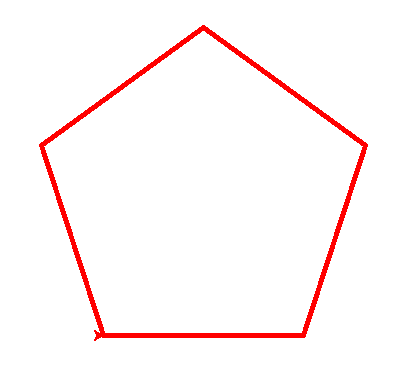
\includegraphics[scale=\myscale,scale=0.25]{screen-turtle-2b}
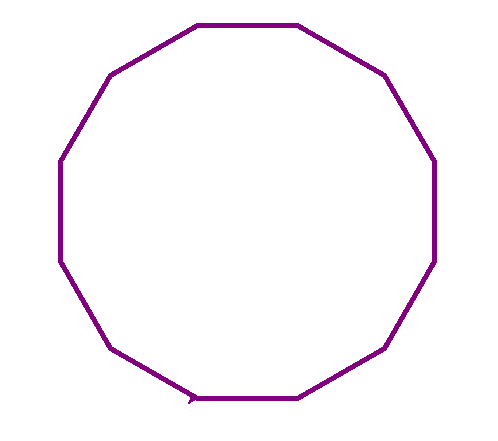
\includegraphics[scale=\myscale,scale=0.25]{screen-turtle-2c}
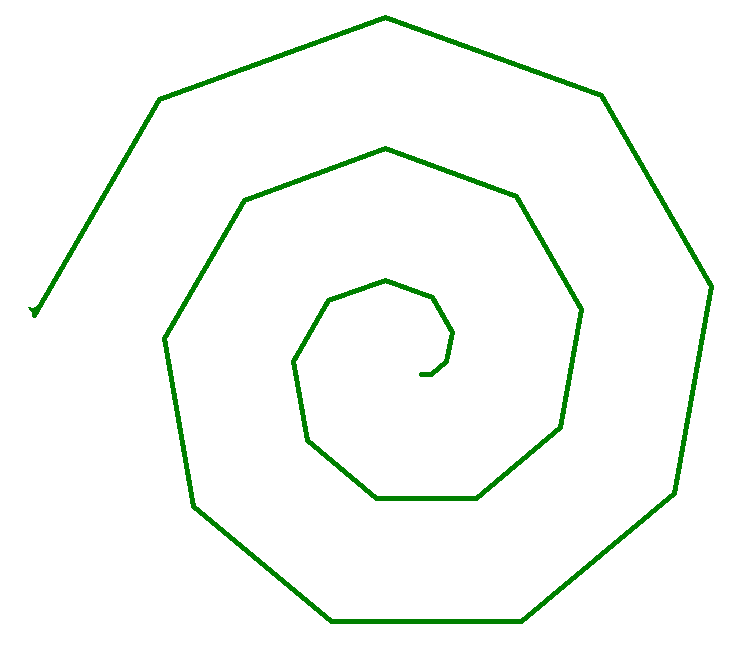
\includegraphics[scale=\myscale,scale=0.2]{screen-turtle-2d}
\end{center}

\begin{enumerate}
  \item \textbf{Pentagon.} Draw a first pentagon (in blue). You have to repeat $5$ times: advance $100$ steps, turn $72$ degrees.
  
  \emph{Hint.} To build a loop, use  
  \mycenterline{\ci{for i in range(5):}}  
   (even if you do not use the variable \ci{i}).
  
  \item \textbf{Pentagon (bis).} Define a variable \ci{length} which is equal to $200$ and a variable \ci{angle} which is equal to $72$ degrees. Draw a second pentagon (in red), this time advancing by \ci{length} and turning by \ci{angle}.
  
  \item \textbf{Dodecagon.} Draw a polygon having $12$ sides (in purple). 
  
  \emph{Hint.} To draw a polygon with $n$ sides, it is necessary to turn an angle of $360/n$ degrees.
  
  \item \textbf{Spiral.} Draw a spiral (in green).
  
  \emph{Hint.} Build a loop, in which you always turn at the same angle, but you move forward by a length that increases with each step.
  
\end{enumerate}
  
\end{activite}



%%%%%%%%%%%%%%%%%%%%%%%%%%%%%%%%%%%%%%%%%%%%%%%%%%%%%%%%%%%%%%%%
% Activity 3
%%%%%%%%%%%%%%%%%%%%%%%%%%%%%%%%%%%%%%%%%%%%%%%%%%%%%%%%%%%%%%%%

\begin{activite}[Function graph]

\objectifs{Goal: draw the graph of a function.}

\begin{center}
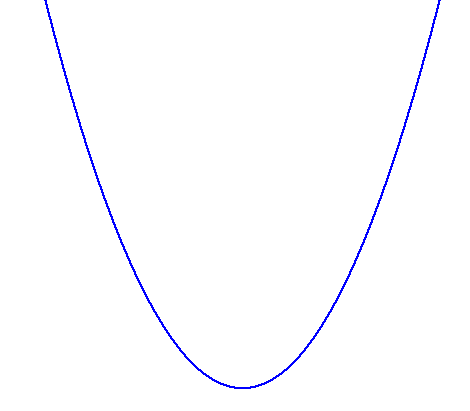
\includegraphics[scale=\myscale,scale=0.4]{screen-turtle-3a}
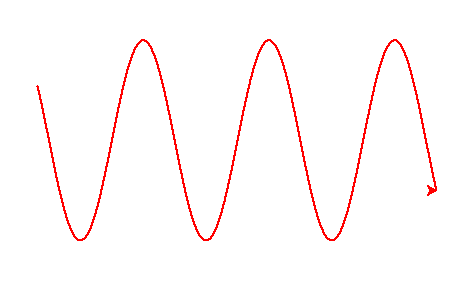
\includegraphics[scale=\myscale,scale=0.4]{screen-turtle-3b}
\end{center}

Plot the graph of the square function and the sine function.

In order to get a curve in the turtle window, repeat for $x$ varying from $-200$ to $+200$:
\begin{itemize}
  \item set $y = \frac{1}{100} x^2$,
  \item go to $(x,y)$.
\end{itemize}

For the sinusoid, you can use the formula 
$$y = 100\sin\left(\frac{1}{20}x\right).$$
  
By default \Python{} does not know the sine function, to use \ci{sin()} you must first import the \ci{math} module:
\mycenterline{\ci{from math import *}}

To make the turtle move faster, you can use the command \ci{speed("fastest")}.
\end{activite}



%%%%%%%%%%%%%%%%%%%%%%%%%%%%%%%%%%%%%%%%%%%%%%%%%%%%%%%%%%%%%%%%
% Activity 4
%%%%%%%%%%%%%%%%%%%%%%%%%%%%%%%%%%%%%%%%%%%%%%%%%%%%%%%%%%%%%%%%

\begin{activite}[Sierpinski triangle]

\objectifs{Goal: trace the beginning of Sierpinski's fractal by nesting loops.}

\index{Sierpinski's triangle}

\begin{center}
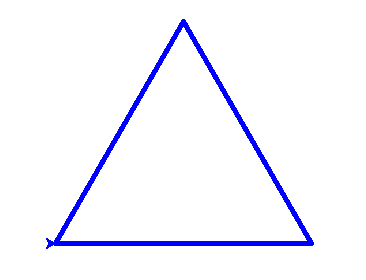
\includegraphics[scale=\myscale,scale=0.3]{screen-turtle-4a}
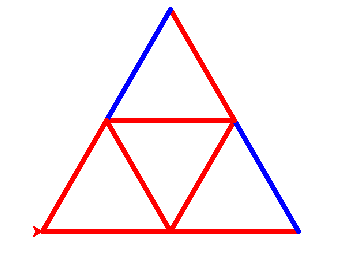
\includegraphics[scale=\myscale,scale=0.3]{screen-turtle-4b}
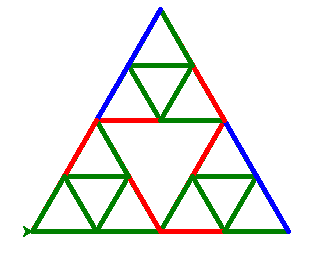
\includegraphics[scale=\myscale,scale=0.3]{screen-turtle-4c}
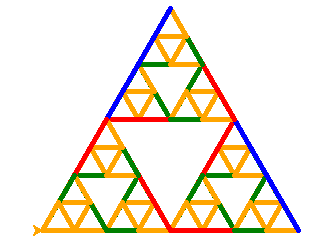
\includegraphics[scale=\myscale,scale=0.3]{screen-turtle-4d}
\end{center}

Here is how to picture the second drawing. Analyze the nesting of the loops and draw the next pictures.

\begin{center}
\begin{minipage}{0.5\textwidth}
\begin{lstlisting}
for i in range(3):
    color("blue")
    forward(256)
    left(120)

    for i in range(3):
        color("red")
        forward(128)
        left(120)
\end{lstlisting}        
\end{minipage}
\end{center}        
\end{activite}



%%%%%%%%%%%%%%%%%%%%%%%%%%%%%%%%%%%%%%%%%%%%%%%%%%%%%%%%%%%%%%%%
% Activity 5
%%%%%%%%%%%%%%%%%%%%%%%%%%%%%%%%%%%%%%%%%%%%%%%%%%%%%%%%%%%%%%%%

\begin{activite}[The heart of multiplication tables]

\objectifs{Goal: draw the multiplication tables.}


We set an integer $n$. We are studying the $2$ table, that is to say 
we calculate $2 \times 0$, $2\times 1$, $2 \times 2$, up to $2 \times (n-1)$. In addition, the calculations will be modulo $n$. We therefore calculate  
$$2 \times k \pmod{n} \qquad \text{ for } k=0,1,\ldots,n-1$$

How do we draw this table?

We place $n$ points on a circle, numbered from $0$ to $n-1$.
For each $k\in \{0,\ldots,n-1\}$, we connect the point number $k$
with the point number $2\times k \pmod{n}$ by a segment. 

Here is the layout, from the table of $2$, modulo $n=10$.

%\begin{center}
% 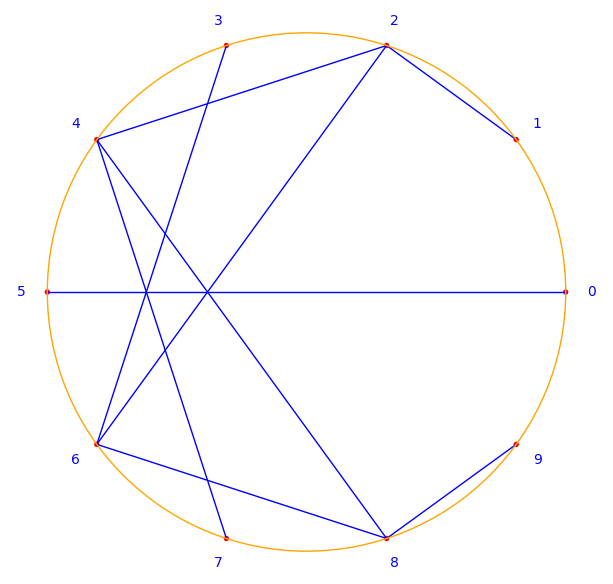
\includegraphics[scale=0.6]{fig-turtle-5a}  
%\end{center}

\myfigure{0.7}{
  \tikzinput{fig-turtle-5a}
}

For example:
\begin{itemize}
  \item the $3$ point is linked to the $6$ point, because $2 \times 3 = 6$;
  \item the $4$ point is linked to the $8$ point, because $2 \times 4 = 8$;
  \item the $7$ point is linked to the $4$ point, because $2 \times 7 = 14 = 4 \pmod{10}$.
\end{itemize}

\bigskip

Draw the table of $2$ modulo $n$, for different values of $n$.

Here is what it gives for $n=100$.

\begin{center}
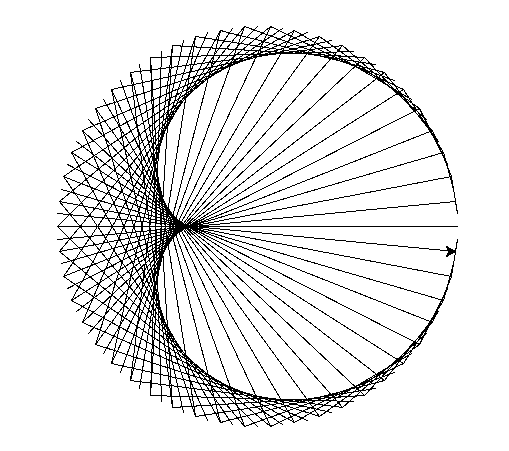
\includegraphics[scale=\myscale,scale=0.5]{screen-turtle-5b}
\end{center}

\emph{Hints.} For calculations modulo $n$, use the expression \ci{(2*k) \% n}.


Here's how to get the coordinates of the vertices. This is done with the sine and cosine functions (available from the \ci{math} module).
The coordinates $(x_i,y_i)$ of the vertex number $i$, can be calculated by the formula:
$$x_i = r \cos\left(\frac{2 i \pi}{n}\right) \qquad \text{ and } \qquad y_i = r\sin\left(\frac{2 i \pi}{n}\right)$$

These points will be located on a circle of radius $r$, centered at $(0,0)$. 
You will have to choose $r$ rather large (for example $r=200$).


\myfigure{0.7}{
  \tikzinput{fig-turtle-5c}
}

\end{activite}

%%%%%%%%%%%%%%%%%%%%%%%%%%%%%%%%%%%%%%%%%%%%%%%%%%%%%%%%%%%%%%%%
%%%%%%%%%%%%%%%%%%%%%%%%%%%%%%%%%%%%%%%%%%%%%%%%%%%%%%%%%%%%%%%%

\begin{cours}[Several turtles]

Several turtles can be defined and move independently.
Here's how to define two turtles (one red and one blue) and move them.

\begin{lstlisting}
turtle1 = Turtle()   # with capital 'T'!
turtle2 = Turtle()

turtle1.color('red')
turtle2.color('blue')

turtle1.forward(100)
turtle2.left(90)
turtle2.forward(100)
\end{lstlisting}

\end{cours}


%%%%%%%%%%%%%%%%%%%%%%%%%%%%%%%%%%%%%%%%%%%%%%%%%%%%%%%%%%%%%%%%
% Activity 6
%%%%%%%%%%%%%%%%%%%%%%%%%%%%%%%%%%%%%%%%%%%%%%%%%%%%%%%%%%%%%%%%

\begin{activite}[The pursuit of turtles]

\objectifs{Goal: draw tracking curves.}

Program four turtles running one after the other:

\begin{center}
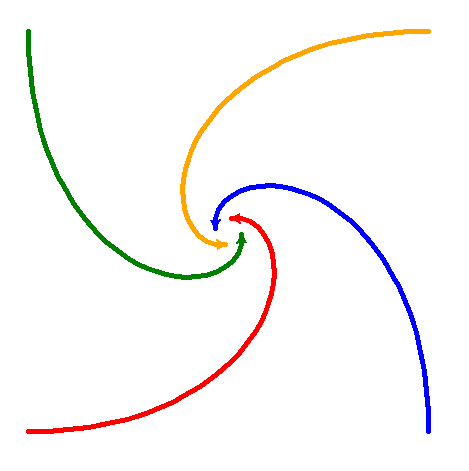
\includegraphics[scale=\myscale,scale=0.5]{screen-turtle-6a}
\end{center}


\begin{itemize}
  \item turtle 1 runs after turtle 2,
  \item turtle 2 runs after turtle 3,
  \item turtle 3 runs after turtle 4,
  \item turtle 4 runs after turtle 1.
\end{itemize}

\bigskip

Here are the starting positions and orientations:
\myfigure{0.9}{
\tikzinput{fig-turtle-6c}
}  


\emph{Hints.}
Use the following piece of code:
\begin{center}
\begin{minipage}{0.5\textwidth}
\begin{lstlisting}
position1 = turtle1.position()
position2 = turtle2.position()
angle1 = turtle1.towards(position2)
turtle1.setheading(angle1)
\end{lstlisting}
\end{minipage}
\end{center}
\begin{itemize}
  \item You place turtles at the four corners of a square, for example at $(-200,-200)$, $(200,-200)$, $(200,200)$ and $(-200,200)$.
  \item You get the position of the first turtle by using 
  \ci{position1 = turtle1.position()}.
  Same for the other turtles.
  \item You calculate the angle between turtle 1 and turtle 2 by the command
  \ci{angle1 = turtle1.towards(position2)}.
  \item You orient the first turtle according to this angle:
  \ci{turtle1.setheading(angle1)}.
  \item You advance the first turtle by $10$ steps.
\end{itemize}

Improve your program by drawing a segment between the chasing turtle and the chased turtle each time.

\begin{center}
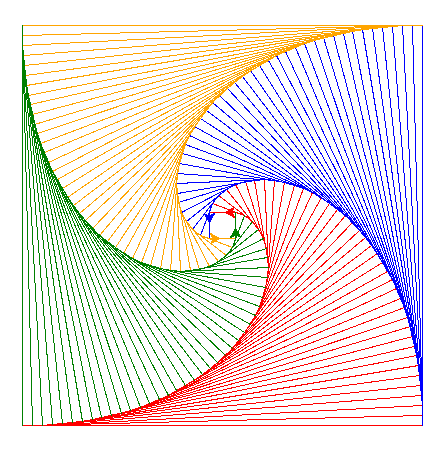
\includegraphics[scale=\myscale,scale=0.5]{screen-turtle-6b}
\end{center}  
\end{activite}

\end{document}


